% mnras_template.tex 
%
% LaTeX template for creating an MNRAS paper
%
% v3.0 released 14 May 2015
% (version numbers match those of mnras.cls)
%
% Copyright (C) Royal Astronomical Society 2015
% Authors:
% Keith T. Smith (Royal Astronomical Society)

% Change log
%
% v3.0 May 2015
%    Renamed to match the new package name
%    Version number matches mnras.cls
%    A few minor tweaks to wording
% v1.0 September 2013
%    Beta testing only - never publicly released
%    First version: a simple (ish) template for creating an MNRAS paper

%%%%%%%%%%%%%%%%%%%%%%%%%%%%%%%%%%%%%%%%%%%%%%%%%%
% Basic setup. Most papers should leave these options alone.
\documentclass[fleqn,usenatbib]{mnras}

% MNRAS is set in Times font. If you don't have this installed (most LaTeX
% installations will be fine) or prefer the old Computer Modern fonts, comment
% out the following line
\usepackage{newtxtext,newtxmath}
% Depending on your LaTeX fonts installation, you might get better results with one of these:
%\usepackage{mathptmx}
%\usepackage{txfonts}

% Use vector fonts, so it zooms properly in on-screen viewing software
% Don't change these lines unless you know what you are doing
\usepackage[T1]{fontenc}

% Allow "Thomas van Noord" and "Simon de Laguarde" and alike to be sorted by "N" and "L" etc. in the bibliography.
% Write the name in the bibliography as "\VAN{Noord}{Van}{van} Noord, Thomas"
\DeclareRobustCommand{\VAN}[3]{#2}
\let\VANthebibliography\thebibliography
\def\thebibliography{\DeclareRobustCommand{\VAN}[3]{##3}\VANthebibliography}


%%%%% AUTHORS - PLACE YOUR OWN PACKAGES HERE %%%%%

% Only include extra packages if you really need them. Common packages are:
\usepackage{graphicx}	% Including figure files
\usepackage{amsmath}	% Advanced maths commands
% \usepackage{amssymb}	% Extra maths symbols

%%%%%%%%%%%%%%%%%%%%%%%%%%%%%%%%%%%%%%%%%%%%%%%%%%

%%%%% AUTHORS - PLACE YOUR OWN COMMANDS HERE %%%%%

% Please keep new commands to a minimum, and use \newcommand not \def to avoid
% overwriting existing commands. Example:
%\newcommand{\pcm}{\,cm$^{-2}$}	% per cm-squared

%%%%%%%%%%%%%%%%%%%%%%%%%%%%%%%%%%%%%%%%%%%%%%%%%%

%%%%%%%%%%%%%%%%%%% TITLE PAGE %%%%%%%%%%%%%%%%%%%

% Title of the paper, and the short title which is used in the headers.
% Keep the title short and informative.
\title[Short title, max. 45 characters]{MNRAS \LaTeXe\ template -- title goes here}

% The list of authors, and the short list which is used in the headers.
% If you need two or more lines of authors, add an extra line using \newauthor
\author[K. T. Smith et al.]
{Ruben Agazzi,Davide Abete, Fabrizio Cominetti
\\
}

% These dates will be filled out by the publisher
\date{Accepted XXX. Received YYY; in original form ZZZ}

% Enter the current year, for the copyright statements etc.
\pubyear{2022}

% Don't change these lines
\begin{document}
\label{firstpage}
\pagerange{\pageref{firstpage}--\pageref{lastpage}}
\maketitle

% Abstract of the paper
\begin{abstract}
this is a simple template for authors to write new MNRAS papers.
The abstract should briefly describe the aims, methods, and main results of the paper. 1525
It should be a single paragraph not more than 250 words (200 words for Letters).
No references should appear in the abstract.
\end{abstract}

% Select between one and six entries from the list of approved keywords.
% Don't make up new ones.

%%%%%%%%%%%%%%%%%%%%%%%%%%%%%%%%%%%%%%%%%%%%%%%%%%

%%%%%%%%%%%%%%%%% BODY OF PAPER %%%%%%%%%%%%%%%%%%

\section{Introduction} 

La realizzazione di questo progetto ha avuto come obbiettivo quello di costruire diversi portafogli, ciascuno sulla base di specifici parametri come $R^2$, $\beta^2$ (rischio sistematico), $\sigma^2$ (rischio totale), al fine di effettuare un confronto in termini di rendimento medio atteso, volatilità e rapporto tra i due, di tutti i portafogli con il principale indice di benchmark dei mercati azionari italiani il FTSE MIB. Per fare ciò siamo partiti da una serie temporale giornaliera riguardante i prezzi di un insieme di stocks e abbiamo considerato come spazio temporale di investimento 5 anni, precisamente dal 2017-06-08 al 2022-06-08. Per ogni stock nell'arco temporale è stata eseguita una regressione dei log-returns ottenuti…(inserire calcolo) su un campione di 180 giorni, ottenendo $R^2$, $\alpha$ e $\beta$. Successivamente, abbiamo selezionato il primo e ultimo 10 per cento delle stocks ordinate in ordine decrescente sulla base ad esempio dell' $R^2$, al fine di costruire un portafoglio caratterizzato da assets di uguale peso, che è stato ribilanciato settimanalmente fino alla fine del campione.
\\Abbiamo calcolato i rendimenti settimanali di ciascuna stock, mediante la differenza tra il log-return corrente e quello della settimana precedente, al fine di calcolare i rendimenti settimanali dell'intero portafoglio come la media pesata dei rendimenti delle singole stock calcolate precedentemente. Inoltre, abbiamo ottenuto i rendimenti settimanali dell'indice FTSE MIB come la differenza tra il rendimento della settimana successiva e quello della settimana precedente. 
Dopo aver fatto queste operazioni, facendo partire il prezzo  da 100 e sommando o sottraendo a questo con cadenza settimanale il rendimento di ciascuna settimana, abbiamo potuto confrontare graficamente con un grafico delle serie storiche i rendimenti settimanali del portafoglio da noi costruito con i rendimenti settimanali dell'indice FTSE MIB, osservando come il rendimento del portafoglio sia prevalentemente maggiore di quello generato dall’indice.
\section{Methods, Observations, Simulations etc.}

Normally the next section describes the techniques the authors used.
It is frequently split into subsections, such as Section~\ref{sec:maths} below.

\subsection{Maths}
\label{sec:maths} % used for referring to this section from elsewhere

Simple mathematics can be inserted into the flow of the text e.g. $2\times3=6$
or $v=220$\,km\,s$^{-1}$, but more complicated expressions should be entered
as a numbered equation:

\begin{equation}
    x=\frac{-b\pm\sqrt{b^2-4ac}}{2a}.
	\label{eq:quadratic}
\end{equation}

Refer back to them as e.g. equation~(\ref{eq:quadratic}).

\subsection{Figures and tables}

Figures and tables should be placed at logical positions in the text. Don't
worry about the exact layout, which will be handled by the publishers.

Figures are referred to as e.g. Fig.~\ref{fig:example_figure}, and tables as
e.g. Table~\ref{tab:example_table}.

% Example figure
\begin{figure}
	% To include a figure from a file named example.*
	% Allowable file formats are eps or ps if compiling using latex
	% or pdf, png, jpg if compiling using pdflatex
	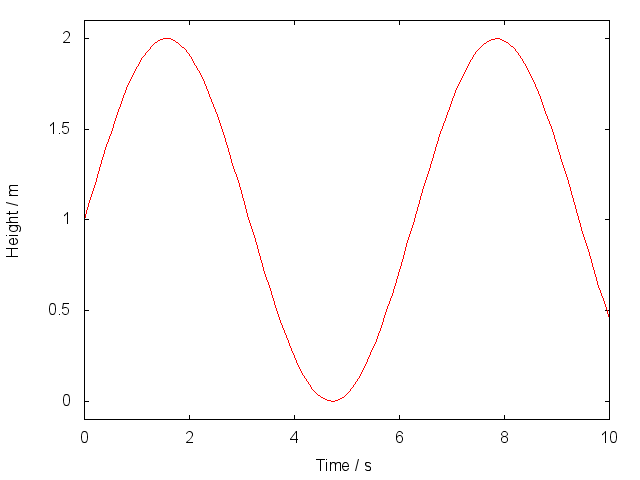
\includegraphics[width=\columnwidth]{example}
    \caption{This is an example figure. Captions appear below each figure.
	Give enough detail for the reader to understand what they're looking at,
	but leave detailed discussion to the main body of the text.}
    \label{fig:example_figure}
\end{figure}

% Example table
\begin{table}
	\centering
	\caption{This is an example table. Captions appear above each table.
	Remember to define the quantities, symbols and units used.}
	\label{tab:example_table}
	\begin{tabular}{lccr} % four columns, alignment for each
		\hline
		A & B & C & D\\
		\hline
		1 & 2 & 3 & 4\\
		2 & 4 & 6 & 8\\
		3 & 5 & 7 & 9\\
		\hline
	\end{tabular}
\end{table}


\section{Conclusions}

The last numbered section should briefly summarise what has been done, and describe
the final conclusions which the authors draw from their work.

\section*{Acknowledgements}

The Acknowledgements section is not numbered. Here you can thank helpful
colleagues, acknowledge funding agencies, telescopes and facilities used etc.
Try to keep it short.

%%%%%%%%%%%%%%%%%%%%%%%%%%%%%%%%%%%%%%%%%%%%%%%%%%
\section*{Data Availability}

 
The inclusion of a Data Availability Statement is a requirement for articles published in MNRAS. Data Availability Statements provide a standardised format for readers to understand the availability of data underlying the research results described in the article. The statement may refer to original data generated in the course of the study or to third-party data analysed in the article. The statement should describe and provide means of access, where possible, by linking to the data or providing the required accession numbers for the relevant databases or DOIs.




%%%%%%%%%%%%%%%%%%%% REFERENCES %%%%%%%%%%%%%%%%%%

% The best way to enter references is to use BibTeX:

\bibliographystyle{mnras}
\bibliography{example} % if your bibtex file is called example.bib


% Alternatively you could enter them by hand, like this:
% This method is tedious and prone to error if you have lots of references
%\begin{thebibliography}{99}
%\bibitem[\protect\citeauthoryear{Author}{2012}]{Author2012}
%Author A.~N., 2013, Journal of Improbable Astronomy, 1, 1
%\bibitem[\protect\citeauthoryear{Others}{2013}]{Others2013}
%Others S., 2012, Journal of Interesting Stuff, 17, 198
%\end{thebibliography}

%%%%%%%%%%%%%%%%%%%%%%%%%%%%%%%%%%%%%%%%%%%%%%%%%%

%%%%%%%%%%%%%%%%% APPENDICES %%%%%%%%%%%%%%%%%%%%%

\appendix

\section{Some extra material}

If you want to present additional material which would interrupt the flow of the main paper,
it can be placed in an Appendix which appears after the list of references.

%%%%%%%%%%%%%%%%%%%%%%%%%%%%%%%%%%%%%%%%%%%%%%%%%%


% Don't change these lines
\bsp	% typesetting comment
\label{lastpage}
\end{document}

% End of mnras_template.tex
